\documentclass{article}  
\usepackage{graphicx}  
\title{Final Assignment}  
\author{Ehsan Rezaei}
\date{Winter of 4031}  
\begin{document}  
\maketitle  
\tableofcontents  
\newpage
\section{Git and GitHub}  
\subsection{Repository Initialization and Commits}  
To set up the repository for this assignment, I followed these steps:  
\begin{itemize}  
    \item Created a GitHub repository named "CW-Final".  
    \item Cloned the repository to my local machine using the command:  
    \begin{verbatim}  
    git clone https://github.com/EhsanRzi/CW-Final.git  
    \end{verbatim}  
    \item Made initial changes to the \texttt{assignment.tex} file and committed them:  
    \begin{verbatim}  
    git add assignment.tex  
    git commit -m "Initial commit"  
    \end{verbatim}  
\end{itemize}
\subsection{GitHub Actions for LaTeX Compilation}  
To set up GitHub Actions, I followed these steps:  
\begin{itemize}  
    \item Created a \texttt{.github/workflows/main.yml} file in my repository.  
    \item Added the following code to automate PDF compilation:  
    \begin{verbatim}  
        name: Release Compiled PDF 
on:
  push:
    tags:
      - '*.*.*'

jobs:
  build_latex:
    permissions: write-all
    runs-on: ubuntu-latest
    steps:
      - name: Set up Git repository
        uses: actions/checkout@v2
      - name: Compile LaTeX document
        uses: xu-cheng/latex-action@v2
        with:
          root_file: main.tex

      - name: Create Release
        id: create_release
        uses: actions/create-release@v1
        env:
          GITHUB_TOKEN: ${{ secrets.GITHUB_TOKEN }}
        with:
          tag_name: ${{ github.ref }}
          release_name: Release ${{ github.ref }}
          draft: false
          prerelease: false

      - name: Upload Release Asset
        id: upload-release-asset 
        uses: actions/upload-release-asset@v1
        env:
          GITHUB_TOKEN: ${{ secrets.GITHUB_TOKEN }}
        with:
          upload_url: ${{ steps.create_release.outputs.upload_url }} 
          asset_path: ./main.pdf
          asset_name: main.pdf
          asset_content_type: pdf
    \end{verbatim}  
    \item Tag the commit to trigger the action:  
    \begin{verbatim}  
    git tag v1.0  
    git push origin v1.0  
    \end{verbatim}  
\end{itemize}     
\section{Exploration Tasks}
\subsection{Vim Advanced Features} 
3 advanced features of Vim: 
\begin{itemize}  
    \item \textbf{Split Windows:} Splitting the screen into multiple windows for simultaneous editing.  
    \item \textbf{Macros:} Recording sequences of commands for automation.  
    \item \textbf{Registers:} Using different registers to store and retrieve text.  
\end{itemize}
\subsection{Memory profiling}  
\subsubsection{Memory Leak}
Memory leaks occur when a program allocates memory but fails to release it after use, leading to reduced performance or crashes.
\subsubsection{Memory Profilers}  
Valgrind is a tool for memory debugging, memory leak detection, and profiling. It helps identify memory issues in applications, ensuring efficient memory management.
\subsection{GNU/Linux Bash Scripting}
\subsubsection{fzf}  
Fuzzy searching allows users to find files or strings based on partial matches, improving search efficiency.
\begin{verbatim}  
ls | fzf 
\end{verbatim}  
allows you to quickly find and choose a file from the current directory interactively, enhancing your efficiency in navigating files in the command line. It's particularly useful when you have a large number of files and directories, as it reduces the need to scroll through the entire list.
\subsubsection{Using fzf to find your favorite PDF}
To list all PDF files:  
\begin{verbatim}  
fd *.pdf  
\end{verbatim}  
Selecting a PDF with fzf:  
\begin{verbatim}  
fd *.pdf | fzf  
\end{verbatim}
\section{Git and FOSS}
\subsection{Issues}
Here is a screenshot of the sample issue created in the GitHub repository.  

\begin{figure}[h]  
  \centering  
  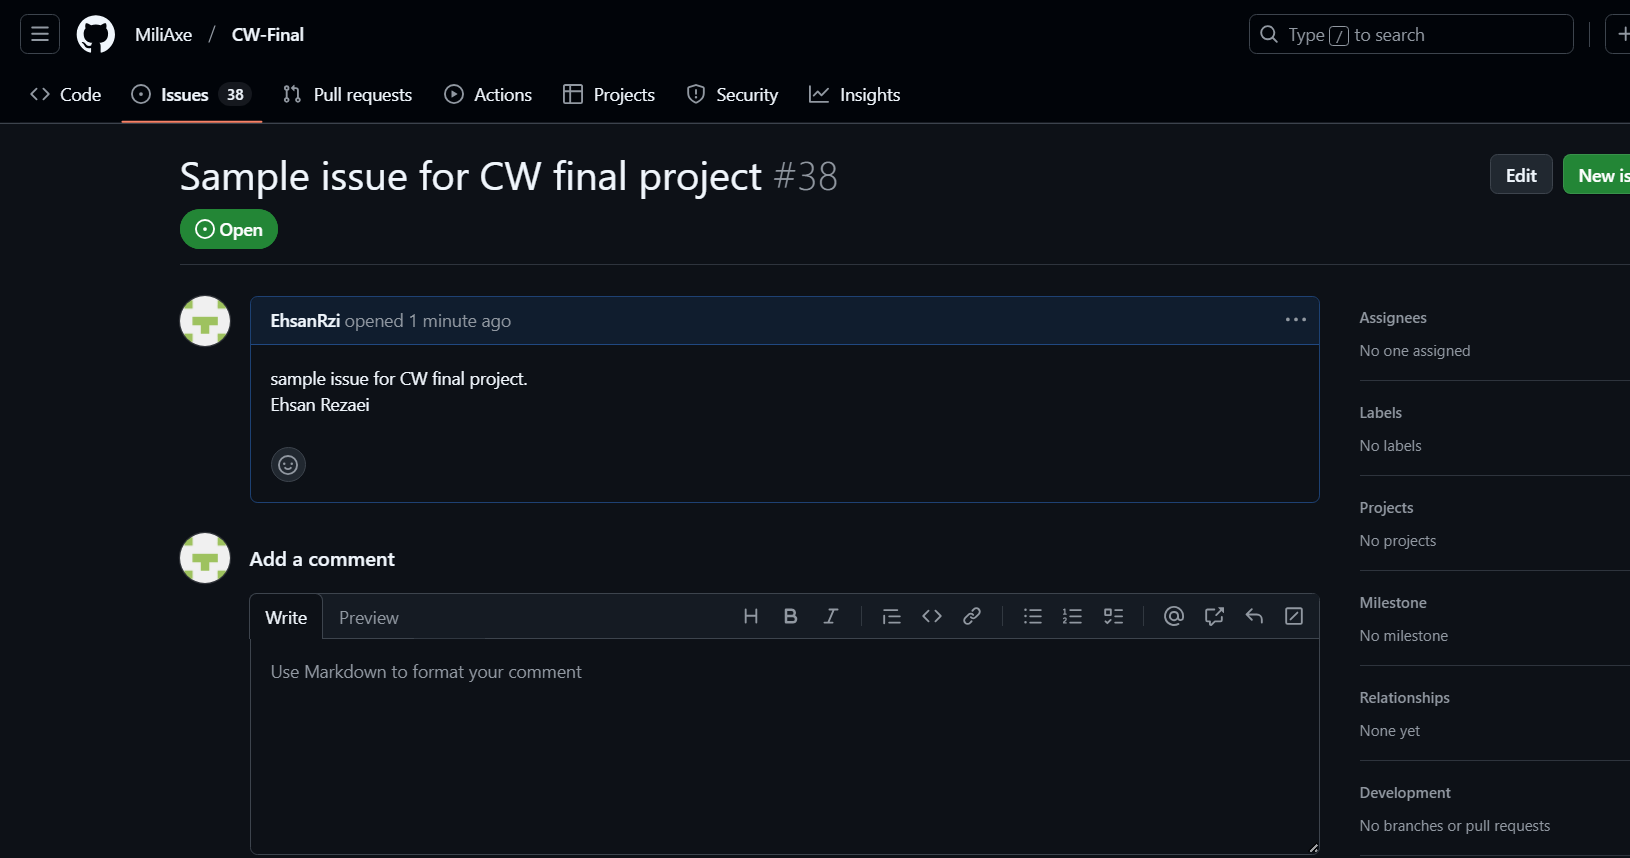
\includegraphics[width=0.8\textwidth]{CW-Final\images\issue_screenshot.png}  
  \caption{Screenshot of the sample issue.}  
  \label{fig:issue_screenshot}  
\end{figure}  
\end{document}  